\section{Objectives and specification mapping}
Lab 10 (PDF pages 39--43) contains four requirements. The first netlist sweeps inverter scales 1--4 and loads 0/0.1/0.2/0.3 pF at a fixed 0.2 ns input-ramp parameter. Its matrix covers fixed-load sizing, fixed-size loading and the joint size/load sweep. The second holds size at one unit and sweeps input ramps 0.2/0.4/0.6/0.8 ns against the same four loads, matching Table 10.1. Both netlists and all 32 cases solved and measured successfully.

\section{Circuit and delay-model derivation}
The unit inverter has $W_p/W_n=1.8/0.6\,\mu$m and $L=0.25\,\mu$m. Size multiplies both widths. An ideal output capacitor sets the load; the zero-load case contains a negligible $10^{-21}$ F numerical capacitor while intrinsic model parasitics remain.

Define mean propagation delay as $z=(t_{pHL}+t_{pLH})/2$. At fixed input ramp, fit $z=A_0+A_1C_L$. Then use load $x$ in pF and PULSE ramp parameter $y$ in ns for the handout's bilinear form
\[z=A+Bx+Cy+Dxy.\]
This is a finite-range approximation, not an exact transistor solution. Separate $t_{pHL}$, $t_{pLH}$ and output rise/fall measurements are all retained in the CSV files.

\section{Simulation setup and measurement definitions}
The separately supplied MOS model is evaluated at 1.0 V and $27\,^{\circ}$C, retaining the handout topology and the comparison conditions below. One volt is a simulation setting, not a device rating established by available model documentation. Numerical results from the handout's older processes are not acceptance targets for this model.

HSPICE S-2021.09 runs with RUNLVL=6. Tables use actual native measurements and figures use actual printed numerical traces. Every variant resets all swept parameters and temperature, avoiding inherited settings from an earlier variant. Completed solutions and measurements do not establish process reliability. Internal warnings in encrypted model blocks remain incompletely visible.
The PULSE SLEW parameter is the linear 0--100\% ramp duration; its 10--90\% duration equals $0.8\times$SLEW. Output transitions use the separate 10--90\% definition. The input period is 25 ns, initial delay 2 ns and high pulse width 10 ns. Transients run for 50 ns with 5 ps printing. Propagation delays use 50\% input/output crossings.

\section{Fixed-input-ramp linear fits}
Units below are ns and pF. Residuals are maximum absolute errors across the four load points.

\begin{center}\small
\begin{tabular}{llll}
\toprule
Size & $A_0$ (ns) & $A_1$ (ns/pF) & Max residual (ps) \\
\midrule
1 & 0.05936 & 3.69754 & 8.96 \\
2 & 0.05939 & 1.87448 & 8.77 \\
3 & 0.05880 & 1.26966 & 7.53 \\
4 & 0.05875 & 0.96623 & 7.18 \\
\bottomrule
\end{tabular}
\end{center}
\begin{figure}[htbp]
\centering
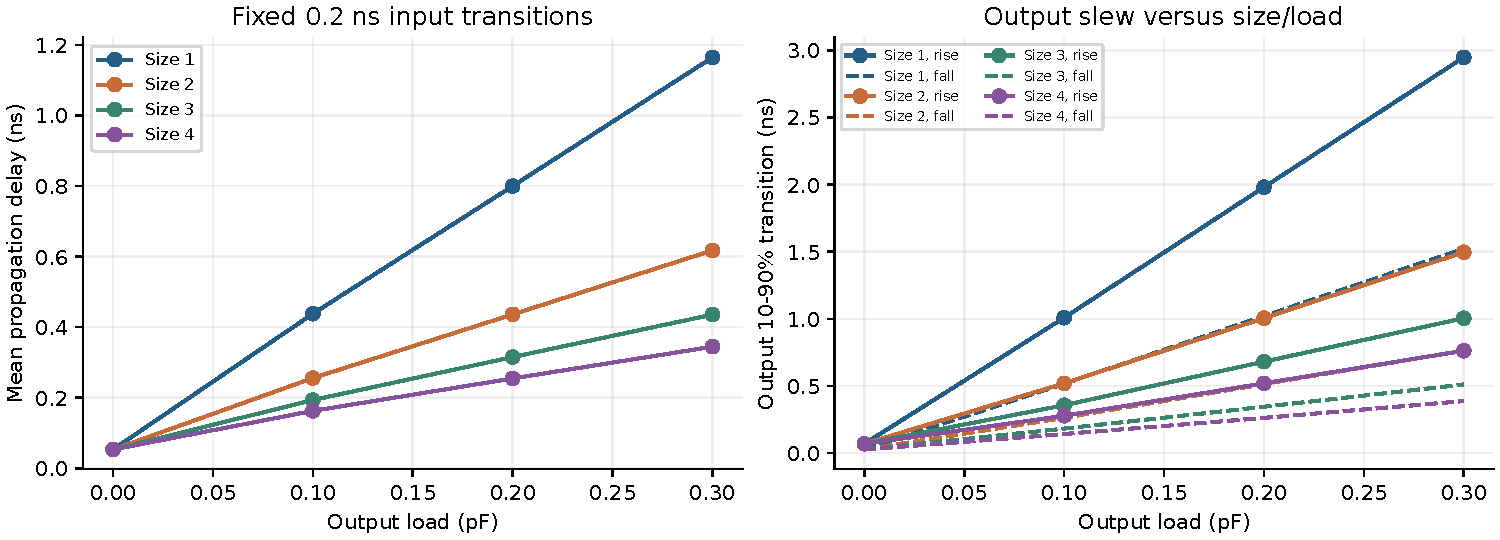
\includegraphics[width=\linewidth]{figures/linear_delay.pdf}
\caption{Load-dependent delay and output rise/fall times at fixed input ramp.}
\end{figure}
\section{Joint load and input-ramp results}
Mean propagation delay in ns; rows are input-ramp parameters and columns are output loads.

\begin{center}\small
\begin{tabular}{lllll}
\toprule
Ramp (ns) & 0 pF & 0.1 pF & 0.2 pF & 0.3 pF \\
\midrule
0.2 & 0.0530 & 0.4381 & 0.8000 & 1.1649 \\
0.4 & 0.0668 & 0.4843 & 0.8484 & 1.2132 \\
0.6 & 0.0768 & 0.5326 & 0.8973 & 1.2600 \\
0.8 & 0.0850 & 0.5808 & 0.9472 & 1.3067 \\
\bottomrule
\end{tabular}
\end{center}
\[z=0.038107+3.583427x+0.109639y+0.556701xy\quad\text{(ns)}.\]
On these same 16 points, load-only RMSE is 51.17 ps. Including input ramp and the interaction term reduces it to 23.64 ps, with maximum residual 52.14 ps. These are in-sample fit errors, not held-out prediction errors.
\begin{figure}[htbp]
\centering
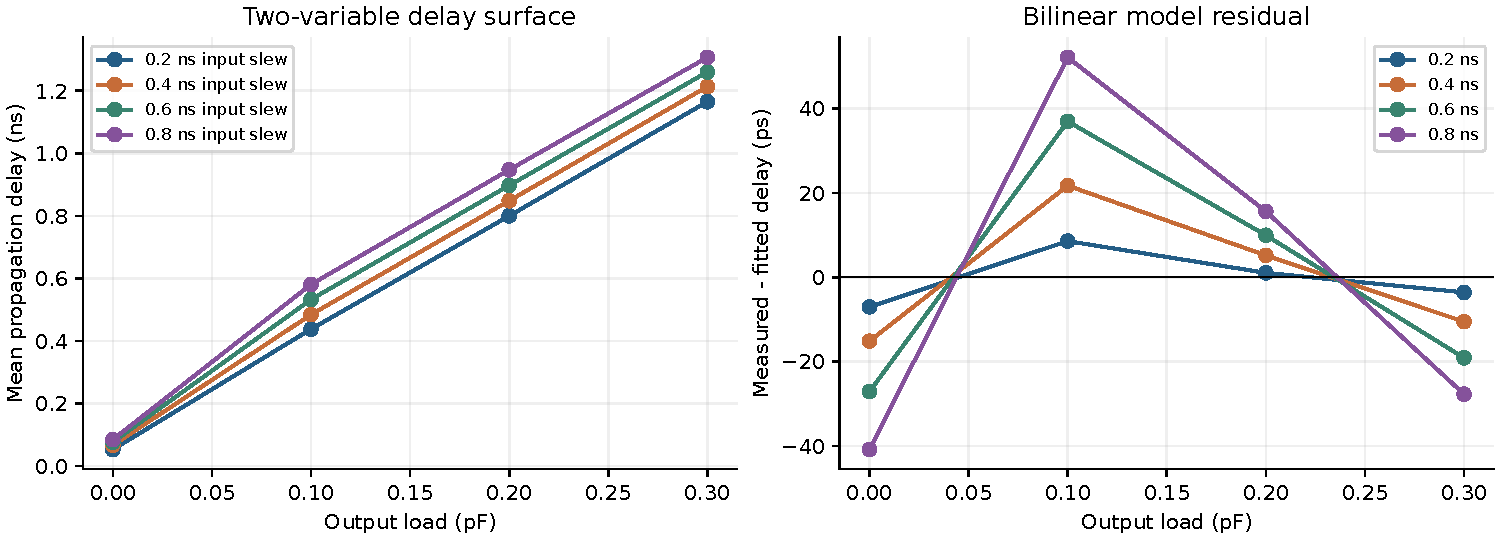
\includegraphics[width=\linewidth]{figures/nonlinear_delay.pdf}
\caption{Input ramp changes the delay surface; the bilinear approximation retains visible residuals.}
\end{figure}
\section{Discussion}
Increasing size lowers delay slope per unit load, from 3.6975 ns/pF at size 1 to 0.9662 ns/pF at size 4. The nonzero intercept combines intrinsic parasitics, finite input ramp and fitting effects; it is not a direct measurement of a single fixed physical capacitance.

At fixed load, slower input ramps increase mean propagation delay, so omitting input slew creates systematic error. The bilinear fit improves average error but retains curvature, particularly at low load and slow ramp. A denser lookup table with interpolation is a reasonable next representation. Connecting measured points in the plots does not validate linear extrapolation outside this range.

\section{Reproducibility files}
The following netlists accompany this report. A comment marks the local model setup; neither the model file nor its path is published. A valid local model configuration must be supplied before execution.
\begin{itemize}
\item \texttt{01\_size\_load.sp}
\item \texttt{02\_slew\_load.sp}
\end{itemize}
The lab results directory contains every case measurement, representative waveform CSV files, derived metrics and a specification manifest. Waveform exports retain at most 2501 uniformly selected samples; direct measurements are not downsampled. Complete original listings remain local.

